\begin{table}[H]
\centering
\begin{tabular}{@{}lll@{}}
\toprule
\textbf{Aspetto} & \textbf{Assione} & \textbf{Elettrone} \\ \midrule
Massa & \(10^{-5}\) eV & 511 keV \\
Lunghezza d'onda & \(0,124\) m & \(2,4\times10^{-12}\) m \\
Comportamento & Onda & Particella \\
Interazione & Molto debole & Elettromagnetica \\
Ruolo in ART-12D & Modo del campo akashico & Ricevitore neurale \\ \bottomrule
\end{tabular}
\end{table}

\subsection{Quali particelle attraversano il suo corpo?}
La materia oscura ha una densità locale di circa 0,3 GeV/cm$^3$ (Read, 2014). La densità numerica dipende però dalla massa, $n = \rho/m$, e il flusso è $\Phi = n v$. Per un modo di $10^{-5}$ eV e $v = 300$ km/s si ottiene:
\begin{equation}
n = \frac{0,3 \times 10^{15}\ \text{eV/m}^3}{10^{-5}\ \text{eV}} = 3,0\times10^{19}\ \text{m}^{-3},
\qquad
\Phi = n v = 9,0\times10^{24}\ \text{m}^{-2}\text{s}^{-1}.
\end{equation}
Per un corpo umano con una superficie di 0,7 m$^2$:
\begin{equation}
\Phi_{\text{body}} = 9,0\times10^{24} \times 0,7 \approx 6\times10^{24} \text{ particles/s}.
\end{equation}
Circa $6\times10^{24}$ particelle al secondo. (La versione 30 affermava $n = 3000$ m$^{-3}$ e $6\times10^8$ s$^{-1}$; quei valori corrispondono a un WIMP di circa 100 GeV, non a un modo di $10^{-5}$ eV.)

\begin{figure}[H]
\centering
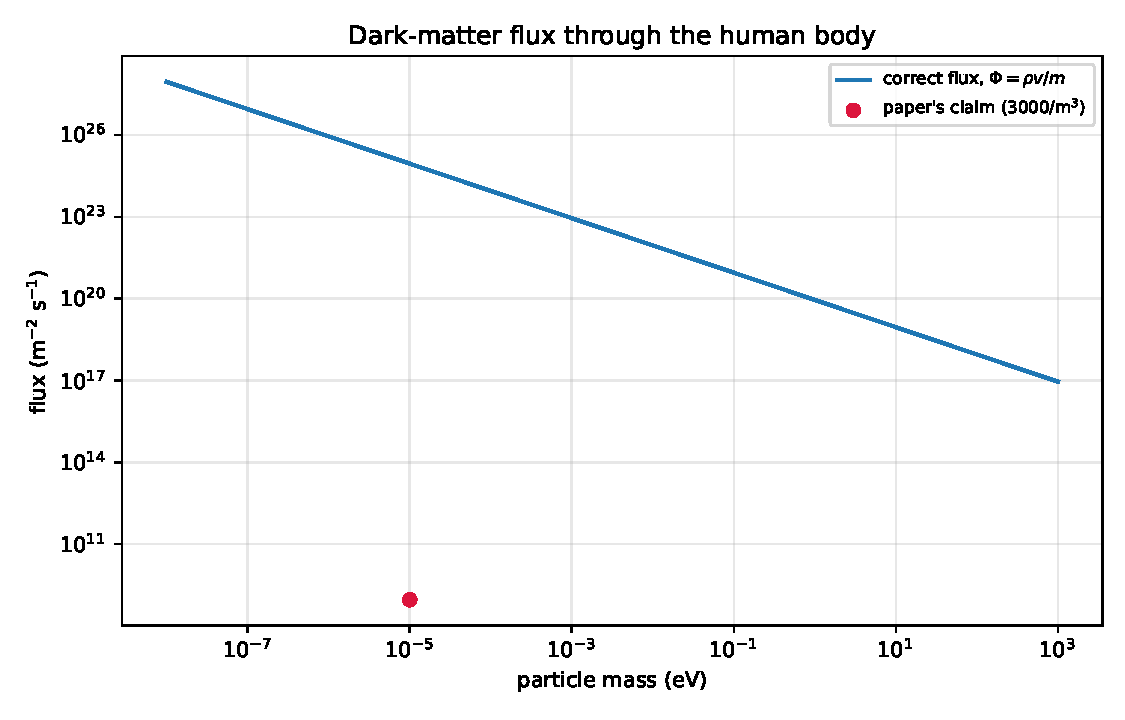
\includegraphics[width=0.82\textwidth]{figures/fig07_flux.pdf}
\caption{Il flusso di materia oscura attraverso il corpo umano in funzione della massa della particella. Il punto rosso segna l'affermazione della versione 30; la curva è il valore corretto per $\rho = 0,3$ GeV/cm$^3$ e $v = 300$ km/s. A $10^{-5}$ eV la differenza è di 16 ordini di grandezza.}
\label{fig:flux}
\end{figure}

\subsection{Che cosa accade a queste particelle?}
La maggior parte lo attraversa senza interagire. Alcune interagiscono con i nuclei atomici: indipendenti dallo spin ($\sim 5$ collisioni/anno), dipendenti dallo spin ($\sim 30$ collisioni/anno). L'effetto sul corpo: radiazione naturale ($\sim 2,4$ mSv/anno); materia oscura ($\sim 10^{-15}$ mSv/anno).

\subsection{Come rileviamo queste particelle?}
Rivelatori diretti: LUX-ZEPLIN (10 tonnellate di xeno) --- sensibilità: $10^{-48}$ cm$^2$. Rivelatori indiretti: Fermi-LAT (cerca raggi gamma da annichilazione), ADMX (cerca assioni). Sezione d'urto: $\sigma \sim 10^{-47}$ cm$^2$. Probabilità di interazione: $P \sim 10^{-22}$.

\subsection{La materia oscura come onda, non come particelle}
Se la materia oscura è un campo scalare, allora non è composta da particelle individuali. È un'onda che riempie l'universo. Formalizzazione: $A(x,t) = \sum_n A_n \cos(\omega_n t + \varphi_n)$.

\subsection{L'analogia dell'albero e del fotone}
Immagini un albero su una spiaggia. Il sole splende. I fotoni partono dal sole con energia $E = h\nu$. Arrivano all'albero. Sono assorbiti da ogni foglia con la stessa energia $h\nu$. Come può un solo fotone arrivare a tutte le foglie con la stessa energia? Se fosse una particella, perderebbe energia a ogni collisione. Ma non lo fa. La risposta è semplice: perché il fotone è un'onda, non una particella. Un'onda non si «consuma» quando attraversa la materia. Si estende su tutto lo spazio. Ogni foglia «vede» l'onda intera. Lo stato del fotone: $|\psi_{\text{photon}}\rangle = \int d^3k \, c(k) |k\rangle$.

\subsection{La dualità onda--particella come meccanismo di attraversamento}
Se la materia non può attraversare tra gli universi (perché richiederebbe energia infinita) e gli universi sono collegati dalla materia oscura, come comunicano? La risposta ART-12D: attraverso la dualità onda--particella. Fase 1: la materia diventa onda. $|\text{particle}\rangle_A \to |\text{wave}\rangle_A$. Fase 2: l'onda attraversa. $|\text{wave}\rangle_A \to |\text{wave}\rangle_B$. Fase 3: l'onda diventa particella. $|\text{wave}\rangle_B \to |\text{particle}\rangle_B$. Fase 4: l'informazione viene trasdotta. $I_A \to I_B$.

\subsection{Lo spettro emotivo umano}
I sentimenti umani si dividono in due grandi categorie: positivi e negativi. Ogni sentimento ha una frequenza caratteristica e un effetto specifico sulla coscienza. Formalizzazione: $S_{\text{total}} = \sum_{i=1}^{48} S_i^{\text{positive}} + \sum_{j=1}^{46} S_j^{\text{negative}}$. Ecco un estratto dalla tabella estesa (la versione completa è nell'appendice B):
\begin{table}[H]
\centering
\begin{tabular}{@{}lll@{}}
\toprule
\textbf{Sentimento} & \textbf{Frequenza dominante (Hz)} & \textbf{Effetto} \\ \midrule
Gioia & 400-600 & Espansione, dinamismo \\
Pace & 200-350 & Calma riflessiva \\
Amore & 200-400 & Emozione profonda \\
Gratitudine & 300-500 & Appagamento \\
Paura & 500-800 & Attiva l'amigdala \\
Rabbia & 600-800 & Furore \\
Tristezza & 400-600 & Malinconia \\
Invidia & 600-800 & Gelosia \\ \bottomrule
\end{tabular}
\end{table}
Le frequenze musicali terapeutiche (432 Hz, 528 Hz, 639 Hz, 741 Hz, 852 Hz, 963 Hz) sono state correlate con le frequenze del campo akashico. I sette sensi umani comprendono cinque fisici (vista, udito, olfatto, gusto, tatto) e due psichici (immaginazione, empatia).

\subsection{Il cuore come modulatore della ricezione}
Il cuore possiede un sistema elettrico proprio (il nodo senoatriale) che genera impulsi indipendentemente dal cervello. Funziona come modulatore della ricezione, non come ricevitore indipendente. Il cervello è il ricevitore principale, il cuore regola la coerenza. Formalizzazione: $C_{\text{coherent}} = C_0 \times (1 + \beta \times HRV)$. Le cifre scientifiche esatte: il cervello consuma circa $20$ W di potenza metabolica, il cuore eroga circa $1-1,3$ W di potenza meccanica, ma produce campi elettrici e magnetici di ampiezza molto maggiore.

\subsection{La parola che può sostituire qualsiasi farmaco}
L'ipotesi: $L_{\text{word-matter}} = g_{CM} A_{\text{meaning}} \psi \psi$. Ciò che la parola può fare: $Effect_{\text{total}} = Effect_{\text{medicine}} + Effect_{\text{word}} + \text{Interaction}$. Ciò che la parola non può fare: non può sostituire gli antibiotici nelle infezioni batteriche, non può sostituire l'insulina nel diabete di tipo 1, non può sostituire la chirurgia nell'appendicite, non può sostituire la chemioterapia nel cancro. Predizione 67: l'effetto della parola.

\newpage
